\documentclass[12pt]{article}

%
% Packages
%

\usepackage{etoolbox}
\usepackage[capposition=top]{floatrow}
\usepackage{graphicx}
%\usepackage{caption}
%\usepackage{subcaption}
\usepackage{placeins}
\usepackage{setspace}
\usepackage{array}
\usepackage{fullpage}
%\usepackage[margin=1.5in]{geometry}
\usepackage{hyperref}
\usepackage{natbib}
\usepackage{microtype}
\usepackage{rotating}
\usepackage{amsmath}
\usepackage{morefloats}
\usepackage{float}
\usepackage{caption}
\usepackage{xcolor}
\usepackage[T1]{fontenc}
\usepackage[utf8]{inputenc}
\usepackage{authblk}
\usepackage{lmodern}

\hypersetup{
    colorlinks,
    linkcolor={black},
    citecolor={black},
    urlcolor={blue}
}
\usepackage{color,colortbl}
\usepackage{geometry}

\newcommand{\red}{\color{red}}
\newcommand{\blue}{\color{blue}}
\newtoggle{final}
\newtoggle{blind}
%\togglefalse{final}
\toggletrue{final}
%\toggletrue{blind}
\togglefalse{blind}

%
% Some utilities
%
%\usepackage{todonotes} % doesn't work - tikz lib too old
% define a mc=margincomment command
\iftoggle{final}{
   \newcommand{\mc}[2]{#1} % make margincomments go away
   \newcommand{\tc}[2]{#1} % make text comments go away
}%else
{
   \newcommand{\mc}[2]{% 1 referenced text 2 initials 3 comment
       \textcolor{blue}{#1}
       \marginpar{\scriptsize\textbf\raggedright\textcolor{red}{#2}}}
  \newcommand{\tc}[2]{\textcolor{blue}{#1}[\textcolor{red}{#2}]}
}

% Asterisk footnote
\makeatletter
\def\@xfootnote[#1]{%
  \protected@xdef\@thefnmark{#1}%
  \@footnotemark\@footnotetext}
\makeatother

%
% Layout
%
\iftoggle{final}{
  \geometry{left=1.0in,right=1.0in,top=1.0in,bottom=1.0in}
}%else
{
  \geometry{left=0.5in,right=2.0in,top=1.0in,bottom=1.0in,marginparwidth=1.5in}
  }


\begin{document}

%Lane Adjustment Ahead: Uncertainty in Commuting Zones, Causes and Impacts
\title{Recalculating ... : How Uncertainty in Local Labor Market Definitions Affects Empirical Findings}

\iftoggle{blind}{\author{[Names of authors suppressed]}}{%
\author[1]{Andrew Foote}
\author[2]{Mark J. Kutzbach}
\author[1,3]{Lars Vilhuber}
\affil[1]{Center for Economic Studies, U.S. Census Bureau}
\affil[2]{Federal Deposit Insurance Corporation}
\affil[3]{Labor Dynamics Institute, Cornell University}
}

\date{August 2017}
\maketitle

\newpage
\setcounter{page}{1}
\begin{abstract}

This paper evaluates the use of commuting zones as a local labor market definition. We revisit Tolbert and Sizer (1996) and demonstrate the sensitivity of definitions to two features of the methodology. We show how these features impact empirical estimates using a well-known application of commuting zones. We conclude with advice to researchers using commuting zones on how to demonstrate the robustness of empirical findings to uncertainty in definitions. \footnote[*]{\iftoggle{blind}{[Acknowledgements redacted]}{The analysis, conclusions, and opinions expressed herein are those of the author(s) alone and do not necessarily represent the views of the U.S. Census Bureau or the Federal Deposit Insurance Corporation. All results have been reviewed to ensure that no confidential information is disclosed, and no confidential data was used in this paper. This document is released to inform interested parties of ongoing research and to encourage discussion of work in progress. }
\iftoggle{blind}{}{Much of the work developing this paper occurred while Mark Kutzbach was an employee of the U.S. Census Bureau.}}\\

Keywords: Local labor markets; commuting; measurement error
\end{abstract}
\vfill

\doublespacing
\pagebreak
%%%%%%%%%%%%%%%%%%%%%%%%%%%%%%%%%%%%%%%%%%%
\section{Introduction \label{sec:intro}}
Local labor markets are an important unit of analysis in labor economics. Theoretical papers emphasize characteristics of a local labor market including common wage and rent levels \citep{Roback1982,Moretti2011} as well as job-finding and unemployment rates \citep{HL2012,SS2014} and often assume fixed or variable costs for transferring jobs or workers between labor markets. In empirical labor economics, researchers interested in estimating the effect of some local, exogenous shock on labor market outcomes must decide how to define the set of affected jobs or workers. Researchers examining labor markets in the United States often turn to one of several standard geographic definitions that are widely known and compatible with publicly available economic data, including: states \citep{BK1992,Wozniak2010,KW2011}, metropolitan areas \citep{BH2000,Card2001,Notowidigdo2011,Diamond2016}, and counties \citep{MRR2015,FGS2015}.

Another labor market definition with advantages for some research topics over the above definitions is commuting zones, which are composed of counties and were originally defined by \citet{TS1996} (henceforth, TS). Commuting zones are similar to metropolitan areas in that they are meant to capture areas of economic integration that do not necessarily conform to regional political boundaries (such as states) \citep{FR2000,FR2010}. Unlike metropolitan areas, commuting zones have no urbanized area size requirements and span the entire United States, allowing researchers to measure effects for the entire country rather than just the set of metropolitan areas (or the complements of metropolitan areas within a state). 

Given these features, commuting zones have been used in a number of influential papers in the labor economics literature, including \citet{ADH2013}, as well as \citet{ChettyHendrenKlineSaez2014}, \citet{AM2015}, \citet{Restrepo2015}, and \citet{Yagan2016}. Despite their widespread use, to the best of our knowledge, the methodology underlying commuting zone definitions and its impact on empirical estimates has not received much scrutiny and many researchers do not consider how findings may be sensitive to design issues. 

Our paper makes two contributions for empirical analysis using commuting zones. First, we describe two methodological issues that researchers should be aware of when they use the commuting zones. We demonstrate the sensitivity of commuting zone definitions to a dissimilarity threshold choice in the clustering process, which governs the number of clusters, and to uncertainty in the underlying worker flows data, which governs the strength of ties between pairs of counties. Second, we show how these methodological issues impact empirical estimates that use commuting zones as the local labor market definition, using a standard analysis that is made in the literature. While both of the issues could, in principle, affect empirical estimates, we find that in this context the dissimilarity threshold choice leads to wider variation in definitions and more substantive differences in estimates. The relative importance of these issues may vary with geographic and empirical context.

Our findings suggest that researchers should consider evaluating the sensitivity of their results, and we propose ways, corresponding to the two issues, that researchers can test if their results are robust to the subjectivity and uncertainty inherent in this definition of local labor markets. These findings are informative to the use of commuting zones for defining local labor markets specifically, but also suggest caution for researchers in general when measuring treatment effects in geographically distinct areas where treatment may not be as discretely related to geography as is implied by the unit of measure. 

The remainder of the paper proceeds as follows. We describe the data we use and the commuting zone definitions and methodology in detail in Section \ref{sec:method}. In Section \ref{sec:dsens} we outline the extent to which commuting zone definitions are sensitive to data inputs and design decisions, and in Section \ref{sec:esens} we discuss how those issues affect empirical estimates and provides guidance for researchers in light of our results. Section \ref{sec:conclusion} concludes and discusses next steps. 




%%%%%%%%%%%%%%%%%%%%%%%%%%%%%%%%%%%%%%%%%%%
\section{Commuting Zone Data and Methodology \label{sec:method}}
The Economic Research Service (ERS), an agency under the U.S. Department of Agriculture for which commuting zones were originally developed, distributes definitions on its website.\footnote{ERS has released commuting zone definitions based on 1980, 1990, and 2000 commuting data. All three definitions are available at http://www.ers.usda.gov/data-products/commuting-zones-and-labor-market-areas.aspx.} Commuting Zones are especially relevant for the economic analysis of rural areas, a focus of ERS, because they include all counties, not just urban counties.

As an alternative to metropolitan statistical areas, or Core Based Statistical Areas \citep{OMB2013}, many researchers examining local labor markets use commuting zones, which also combine sets of counties based on commuting flows, because they cover the entire country. However, few researchers are familiar with the methodology used to develop these zones. To that end, this section describes the methodology used by \cite{TS1996} in developing the zones.\footnote{The methodology was originally used in \cite{TK1987}, but the 1996 paper is much more
widely cited, and the zones from that paper are the ones most commonly used. For more background on the development of commuting zones, see \cite{FowlerRhubartJensen2016}.}

We describe two especially important design components: the dissimilarity matrix, which measures how ``far'' nodes are from one another, and the clustering method, which decides how nodes are assigned to groups.

\subsection{Dissimilarity Matrix}

The dissimilarity matrix, $d$, is a representation of the relative distance between all pairs of $N$ counties. TS calculate $d$ (or conversely, the similarity matrix $p$), where an entry $D_{ij}$ is the dissimilarity of county $i$ from county $j$, as below:\footnote{The clustering method used requires a dissimilarity matrix; one is just the complement of the other, by element, so $d_{ij}=(1-p_{ij})$.}

\begin{equation}\label{eqn:diss}
d_{ij} = 1- \frac{f_{ij}+f_{ji}}{\min(rlf_{i},rlf_j)}
\end{equation}

In the above equation, $f_{ij}$ is the flow of commuters who live in county $i$ and work in county $j$ and $f_{ji}$ is the opposite flow. The resident labor force in county $i$ is $rlf_i = \sum_{j=1}^{N} f_{ij}$ (including $f_{ii}$), with a corresponding calculation for county $j$. Normalizing flows with the minimum resident labor force of a pair upweights the association of outlying areas with metropolitan cores. Note that disimilarity is symmetric, so $d_{ij}=d_{ji}$.

TS1996 compute $d$ using flows from the 1990 Journey-to-Work data, which tabulates the commuting information from the 1990 Census Long-form \citep{Census1990jtw}.\footnote{Journey to Work data on county to county commuting flows are available for the 1990 Census, the 2000 Census, and 5-year samples of the American Community Survey at \url{https://www.census.gov/hhes/commuting/data/commutingflows.html}.} The Census Bureau estimates county-to-county flows among 3,141 county equivalents for persons age 16 and older who reported being employed in the week prior to April 1, 1990.\footnote{Employment status is based on responses to the question ``Did this person work at any time LAST WEEK?'' Place of work is geocoded using the response to ``At what location did this person work LAST WEEK?'' Residence location is compiled from the mailing frame of the Census.} The Economic Research Service maintains the 1990 commuting zones.%
% This is a repeat from further up
%\footnote{Other releases of commuting zones have used 1980 and 2000 data. All three are available at \url{http://www.ers.usda.gov/data-products/commuting-zones-and-labor-market-areas.aspx}.} 

\subsection{Clustering Method}

After constructing this dissimilarity matrix, TS use it as an input into their clustering method. In general, data scientists use clustering methods to assign interrelated items, or items with similar features, into groups. In their application, TS use the average-linkage hierarchical clustering algorithm (PROC CLUSTER in SAS software).\footnote{The hierarchical clustering for this paper using PROC CLUSTER was generated using SAS software, Version 9.2 of the SAS System for Unix. Copyright \copyright 2009 SAS Institute Inc. SAS and all other SAS Institute Inc. product or service names are registered trademarks or trademarks of SAS Institute Inc., Cary, NC, USA.}
The hierarchical clustering method uses the dissimilarity matrix in the following way. To begin, every county is its own cluster. Then, it finds the lowest value $d_{ij}$ in the dissimilarity matrix, and combines those two counties together. It then recalculates a dissimilarity value between the new cluster and all other clusters. At the cluster level, the dissimilarity for a pair of clusters, $C_K$ and $C_L$, is calculated as the average of dissimilarity among all pairs of counties between the clusters, written:

\begin{equation}\label{eqn:diss_cluster}
D_{KL} = \frac{1}{N_K N_L} \sum_{i \in C_K} \sum_{j \in C_L} d_{ij},
\end{equation}
%notation now mostly matches SAS website, with capitals for clusters and lower case for nodes: https://support.sas.com/documentation/cdl/en/statug/63347/HTML/default/viewer.htm#statug_cluster_sect012.htm

where and $d_{ij}$ is calculated as in Equation \ref{eqn:diss} and $N_K$ and $N_L$ are the count of nodes, or counties in this case, in each cluster. The process continues joining clusters (including singletons with only one county) with the lowest dissimilarity, $D_{KL}$ until all nodes are clustered. The designer may set a stopping threshold by choosing a maximum ``cutoff'' height, $H$, such that if $D_{KL}>H$, then $K$ and $L$ do not merge. TS1990 uses clusters with distances up to $0.98$.

We illustrate this process in Appendix Figure \ref{fig:caliclusters}, which, displaying only California, shows the hierarchical progression of how counties are clustered together. In the top left-hand corner, only a few counties have joined at a height of $H=0.80$. As we increase the height to 0.88 and to 0.96, more counties are joined together. Finally, at a height of 1, almost all the counties have merged together, forming one large cluster and a few much smaller clusters.

\subsection{Our Replication}
\FloatBarrier

In order to replicate the clustering result in TS, which we refer to as TS1990, we use the 1990 Census JTW data and the methodology described above, with one important exception. Because of computing power constraints in 1996, TS divided the country into six overlapping regions and performed the clustering algorithm on each region separately, and then manually resolved conflicts in overlapping regions. This decision has two consequences for users: first, while the height cutoffs across regions are the same, a step in the algorithm that normalizes distances to unit mean will operate differently across regions. Second, it induces some undocumented subjectivity, since conflicts in cluster assignment for counties in the overlapping regions are inevitable.

Rather than follow their methodology of dividing the country into regions, which required a subjective expert review, we run the hierarchical clustering algorithm on the entire country. We choose a height cutoff, 0.9385 (compared to 0.98), that most closely replicates their original zones in terms of size distribution, though it results in 755 zones (compared to 741). We find that the clustering algorithm, when attempting to produce the same cluster count as TS1990 with a national run, retains a residual cluster that spreads across many states. Only with the lower cluster height, and more clusters, does the residual cluster break up. We leave evaluation of alternate clustering methods for future work, with the emphasis in the present analysis on the sensitivity of estimates to zone definitions. We also note that this residual cluster is a feature of the hierarchical procedure, which chooses things which are locally optimal, but can diverge from global optimum rather starkly.\footnote{We show an example of such a map, using a cutoff of 0.945, in Figure \ref{fig:highcutoff} in the Appendix.}

TS1990's zones and our replication are in Figure \ref{fig:czreplication}, and our summary statistics comparing the zones are in Table \ref{tab:replication}. As would be expected given the difference in cluster count, the allocation of counties to clusters varies across the definitions. Our replication has more evenly sized clusters with fewer clusters made up of a single county. We refer to our replication as FKV1990.
 
\begin{figure}[tbh]\centering
\begin{tabular}{cc}
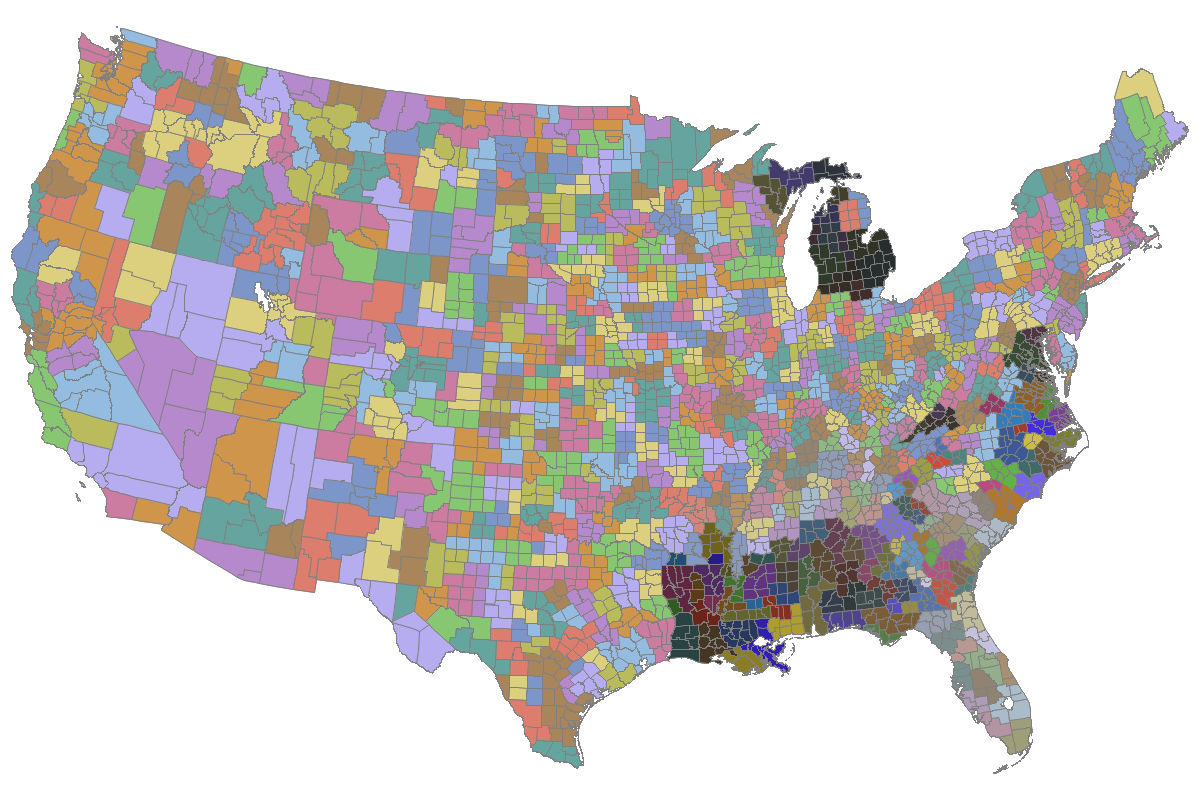
\includegraphics[scale=0.25]{./figures/commutingzones.png}&
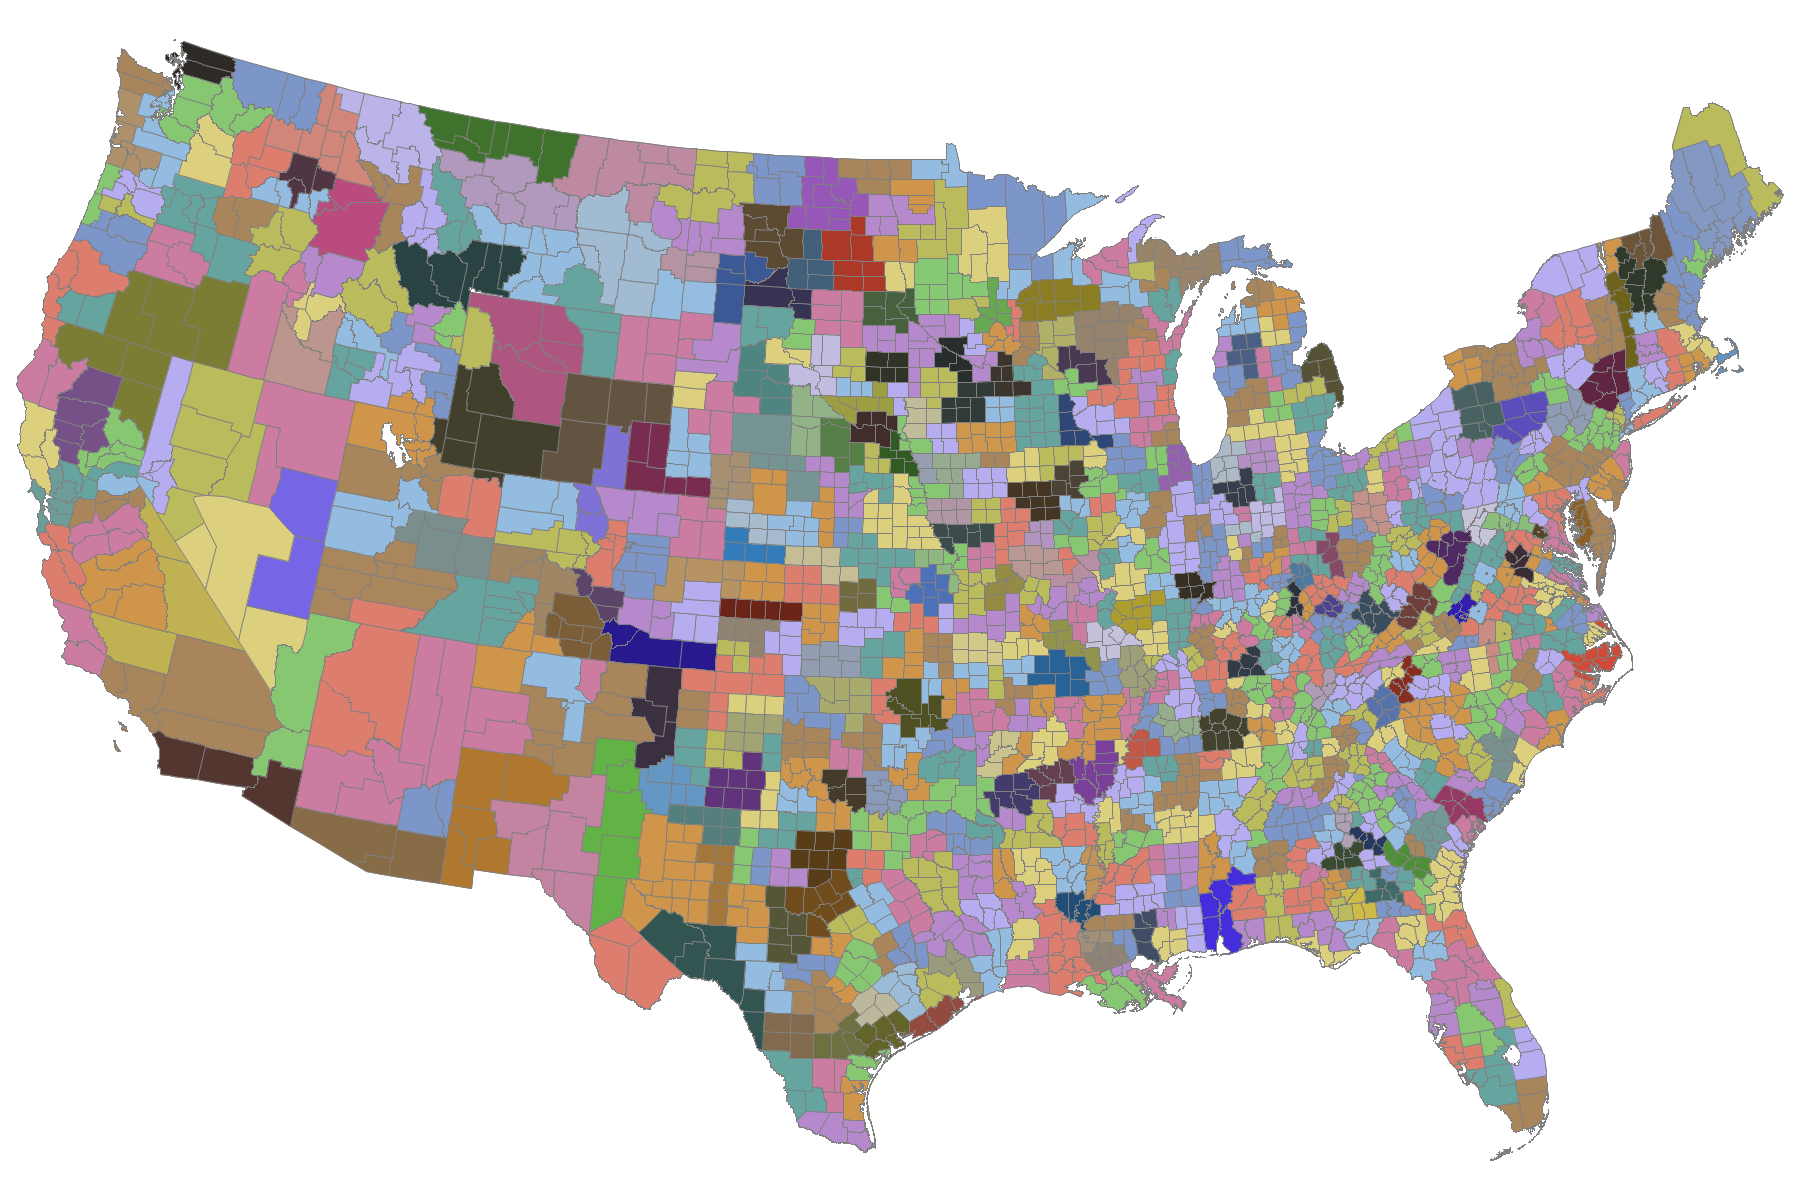
\includegraphics[scale=0.17]{./figures/1990_replicationmap_1.png}\\
Commuting Zones - TS1990 & Replication of Commuting Zones - FKV1990 \\
\multicolumn{2}{l}{\footnotesize \textit{Notes:} Author's calculations using the 1990 Census Journey to Work Tables. More detail in text}\\
\end{tabular}
\caption{Replication of Commuting Zones from TS1996: County Mapping \label{fig:czreplication}}
\end{figure}

% source: name of SAS program
% Last updated:

\begin{table}\centering
\caption{Replication of TS1990 Commuting Zones: Summary Statistics \label{tab:replication}}
\begin{tabular}{lcc}
\hline\hline
       & TS1990 &  FKV1990  \\
       \hline
Mean Cluster Size &  4.24  & 4.16 \\
Median Cluster Size & 4 & 4 \\
Number of Clusters & 741 & 755  \\
Number of Singletons & 62 &  12 \\
Share of Population Mis-matched & \multicolumn{2}{c}{0.17}\\
\hline
\multicolumn{3}{p{4in}}{\footnotesize \textit{Notes}: Both TS1990 and FKV1990 are based on JTW tabulations from the 1990 Census. Summary statistics for TS1990 are from Table 8 of TS.}\\
\end{tabular}
\end{table}


%Mark will look at writing a more efficient macro for this


%%%%%%%%%%%%%%%%%%%%%%%%%%%%%%%%%%%%%%%%%%%
\section{Design Sensitivity \label{sec:dsens}}
While commuting zones are used by researchers as a convenient measure of local labor markets, they have a number of shortcomings for empirical research that are not regularly discussed in the literature. In this section, we evaluate the sensitivity of commuting zone definitions, focusing on two aspects of the TS1990 methodology. First, we show that there is substantial ambiguity over the choice of when to stop merging the clusters, and that small changes in the chosen cutoff height can affect the number and size of the clusters. Second, we show that if there is uncertainty in the input data, the resulting commuting zone definitions can vary substantially. Overall, this uncertainty and subjectivity in the commuting zone definitions contributes to conventional standard errors understating the true level of uncertainty in the estimates, which we show when we return to this issue with our empirical replication in the next section.

\subsection{Choosing Cluster Height}
\FloatBarrier
One sensitive feature of the methodology used by TS is choosing the cutoff value above which no clusters can form, or the maximum dissimilarity, which determines the number of clusters. \cite{TK1987} describe the algorithm for choosing a cutoff value as follows (see page 15): ``As a rule of thumb, a normalized average distance of 0.98 was considered sufficient distance between sets of counties to treat them as separate [Labor Market Areas].'' The article does not provide an analysis of the sensitivity to changing the cutoff marginally up or down. \cite{TS1996}, in an effort to minimize methodological differences between commuting zones for 1980 and 1990, use the same cutoff with no further evaluation for the 1990 data. In this subsection, we investigate how sensitive the resulting clusters are to the choice of the cutoff value.

\begin{figure}
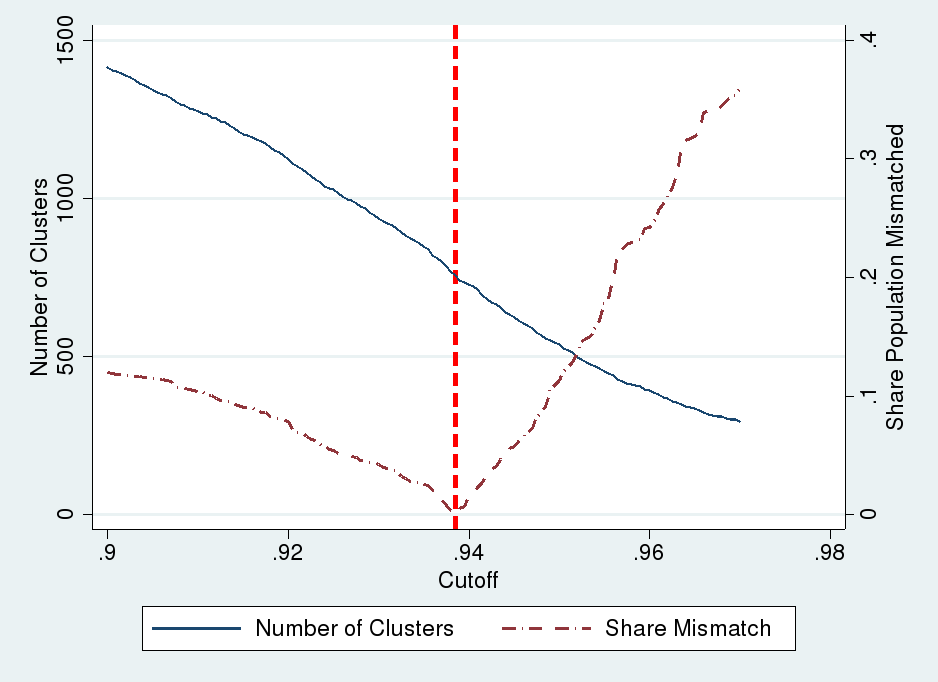
\includegraphics[scale=0.25]{./figures/numclus_cutoff.png}
\caption{Effect of Cluster Height on Number of Clusters \label{fig:cutoff_count}}
\emph{Note:} Authors' calculations using methodology outlined in Section \ref{sec:method}.
\end{figure}

Figure \ref{fig:cutoff_count} shows the number of clusters that form at various height cutoffs using the 1990 JTW data, with the vertical line indicating the cutoff value we chose to replicate TS1990 (0.9385). The key takeaway from this figure is that it is theoretically ambiguous where a researcher should choose to stop merging clusters.\footnote{Decisions on clustering methods, clustering counts, and validation criteria depend on the application and are inherently somewhat subjective. Because clustering is an unsupervised method, there may be no indication of the ideal number of clusters \citep{HBV2001}.} Additionally, increasing or decreasing the cutoff has implications for the number of resulting clusters. Decreasing it to 0.9375 increases the number of clusters by 29, while using a cutoff of 0.93995 cause the number of clusters to decrease by 20. We also graph the share of the population that is in a different cluster than the replicated clusters, to illustrate how assignment changes further away from the cutoff. As we noted earlier, one particular issue with the methodology is that for cutoffs to the right of the vertical line, a large residual cluster forms, which contributes to the steeper slope in the share of the population mismatched.

%As we described above, the measurement error in commuting flows causes some uncertainty in terms of the true dissimilarity matrix, and hence the true cluster heights. Because of the presence of a strict cutoff, some clusters that would have formed if $D_{ij}$ were measured without error do not form, and vis-versa. 

More broadly, TS provide no empirical guidance for choosing the optimal cutoff and cluster size other than referring to expert knowledge. While outside the scope of the current paper, future work may explore data-driven methods to determine whether there is an optimal number of clusters for certain uses. as well as clustering methods that provide more globally optimal clusters.

\subsection{Sensitivity of Clustering Results to Underlying Error}
\FloatBarrier

Another potential sensitivity of the commuting zone methodology is the use of the Journey to Work data, which is subject to sampling error. We analyze the extent to which the outputs of the TS methodology are sensitive to errors in this data. First, recall Equation \ref{eqn:diss} for the entries of the dissimilarity matrix. If $f_{ij}$ is measured without error, then the distance between counties $i$ and $j$ is also measured without error. However, if the flows are measured with error, $\epsilon_{ij}$, then observed flows may be defined as $\hat{f}_{ij}=f_{ij}+\epsilon_{ij}$. In this way, our observed $\hat{rlf}_{i}$, $\hat{rlf}_{j}$, and $\hat{d}_{ij}$ would also include error. We express this assumption below (assuming without loss of generality that $rlf_i < rlf_j$):

\begin{align*}
\hat{d}_{ij} &= 1 - \frac{\hat{f}_{ij} + \hat{f}_{ji}}{\hat{rlf}_i} \\
&= 1- \frac{f_{ij} + f_{ji}}{rlf_{i} + \sum_j \epsilon_{ij}} +  \frac{\epsilon_{ij} + \epsilon_{ji}}{rlf_{i} + \sum_j \epsilon_{ij}}
\end{align*}

Even if $E[\epsilon_{ij}]=0$, that does not imply that $E[\hat{d}_{ij}] = d_{ij}$. Furthermore, we cannot rely on the limit properties of the error distribution, because we only have one realization of the commuting flow, which is calculated from survey responses. Additionally, we know that $\epsilon_{ij}/f_{ij}$ is larger for small flows. Errors will increase $d_{ij}$ for some small counties and decrease it for others. Because of the hierarchical nature of the clustering method, this error will affect the formation of all other clusters in the data.\footnote{Additionally, because heights are normalized in the procedure, it also affects where the effective cutoff is, even for counties unaffected by errors in flows.}

To demonstrate how this measurement error affects the outcome of the clustering procedure, we project the published margins of error (MOE) from the 2009-2013 ACS Journey to Work data onto the 1990 Journey to Work data (which does not publish margins of error). \footnote{To project MOE to 1990, we calculate a ratio, $MOE_{ij}/f_{ij}$, representing the degree of uncertainty for a flow in ACS. To reflect the range of MOEs across similar flows, we calculate the mean and standard deviation of these ratios within flow size bins, defined by 1990 flow percentile, of: 0-50; 50-90; 90-95; 95-99; and 99+. For each 1990 flow, we draw a ratio from the distribution in the corresponding bin. Note that the Census Long form is designed to be a one-in-six sample for one year, while the ACS 5-year summary is designed to 5 years with a one-in-fifty sample each year. The smaller sample size typically results in higher margins of error in the ACS for comparable statistics. The uncertainty implied by our implementation likely overstates the underlying MOEs in the 1990 JTW. For more information on the construction of the ACS MOEs, refer to \url{https://www2.census.gov/programs-surveys/acs/tech_docs/accuracy/MultiyearACSAccuracyofData2013.pdf}, pages 10-12.} Using these estimated MOEs, we then obtain different realizations of the commuting zones in the following way:

\begin{enumerate}
	\item For each origin-destination pair ($i,j$), we draw $\epsilon_{ij}$ from a normal distribution with mean 0 and standard deviation $MOE_{ij}/(1.645)$, since the MOE is scaled to be the 90\% confidence interval.\footnote{In doing this, we assume that $\epsilon_{ij} \perp \epsilon_{ik} \forall k$, for simplicity. In reality, it is likely that $corr(\epsilon_{ij},\epsilon_{ik})<0$, which means in our setting that we are understating the error by treating them as independent. In the JTW data, there are likely some origin-destination pairs that are not reported due to the sample design. In our current resampling approach, we only resample from non-zero flows in the data. A more complete approach would be to model the likelihood that a zero reported is actually a positive flow, and resample accordingly. This modeling is beyond the scope of this paper. For more detail on the 1990 Decennial Census sample design, consult \url{https://www2.census.gov/prod2/decennial/documents/D1-D90-PUMS-14-TECH-01.pdf}.}
	\item Calculate the new flow value, $\hat{f_{ij}} = f_{ij} + \epsilon_{ij}$, with negative values set to zero.\footnote{Many small flows, 65 percent, are not distinguishable from zero and are at risk to be censored, but these tend to be small flows and account for only 1.7 percent of jobs.}
	\item Re-calculate each dissimilarity matrix entry $\hat{d}_{ij}$. 
	\item Re-run the hierarchical clustering procedure, using the same cutoff as the replication.
	\item Store the new clusters, and calculate the following statistics: average number of counties in a cluster; number of clusters; and total number of counties in a different cluster than the one they were originally assigned.
\end{enumerate}

We iterate over this procedure 1000 times in order to obtain distributions for these statistics. These graphs are shown in Figure \ref{fig:sensitivity}, where the red vertical dashed lines are the values for our replication, FKV1990, obtained using the published 1990 data. The figures show that the average cluster size varies considerably from the result the published figures would yield. The share of the population that is mismatched turns out to be less than 1\% of the US population, even in the most varied cases.

\begin{figure}
\caption{Results from Re-sampling Commuting Flows  \label{fig:sensitivity}}
\begin{tabular}{ccc}
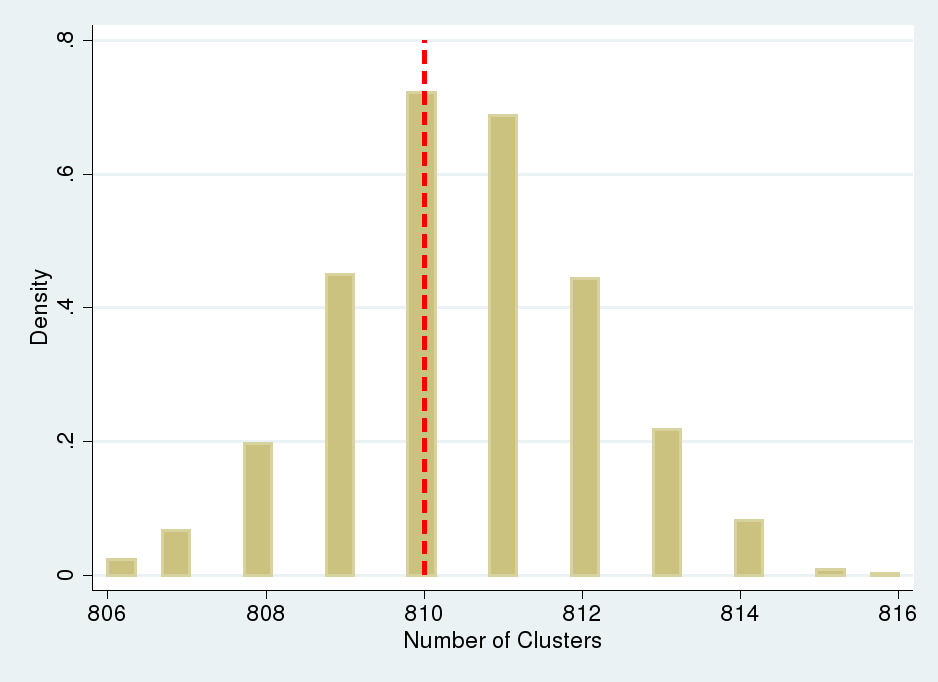
\includegraphics[scale=.15]{./figures/numclusters_jtw1990.png}& 
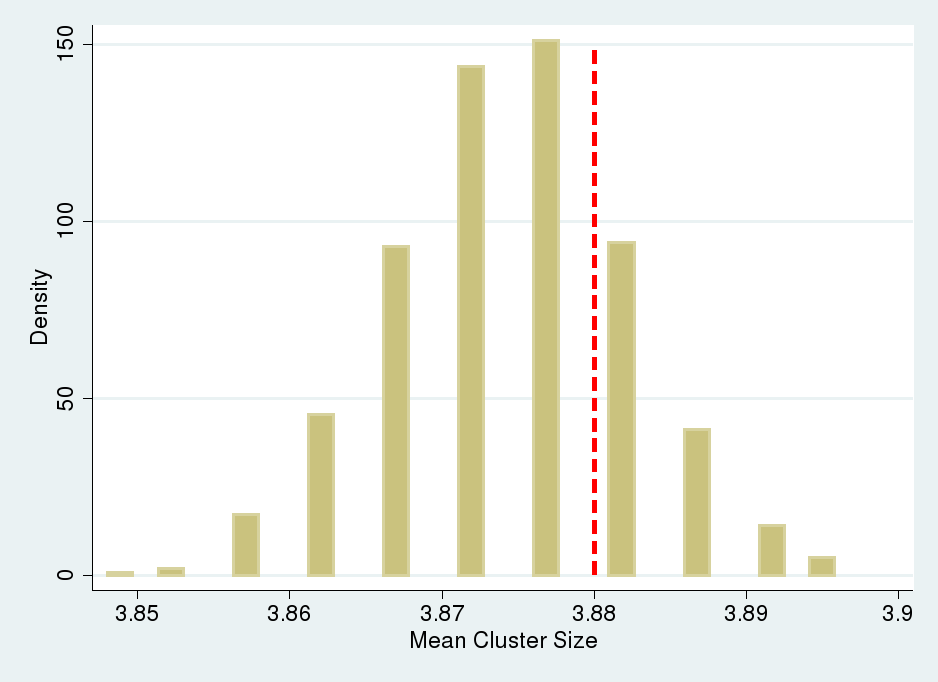
\includegraphics[scale=.15]{./figures/meanclussize_jtw1990.png}&
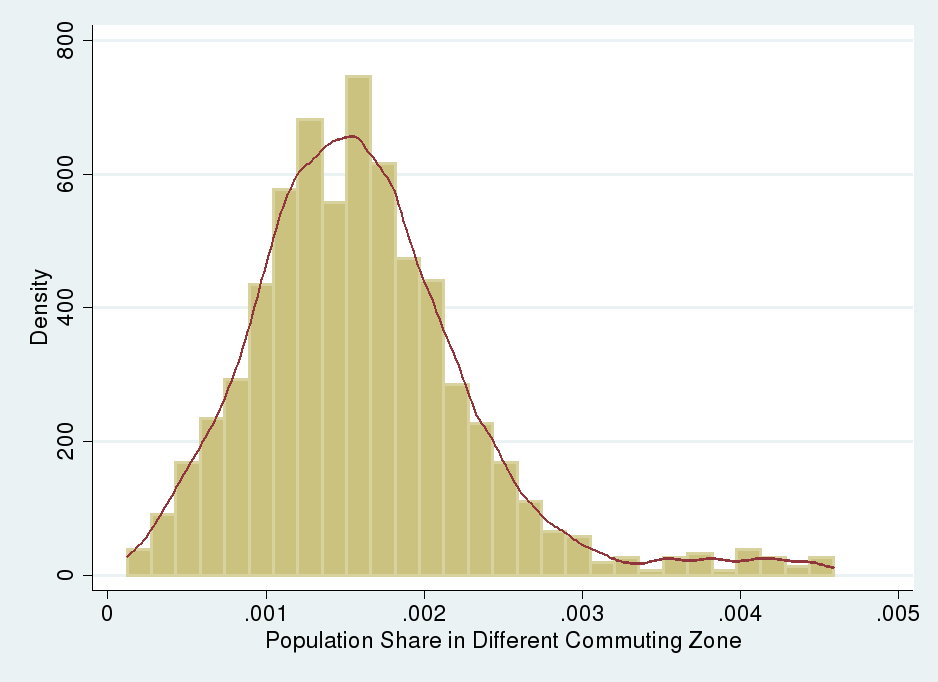
\includegraphics[scale=.15]{./figures/mismatch_jtw1990.png} \\ 
(a) Number of clusters & (b) Average Number of Counties & (c) Share of Mismatched Population \\
\end{tabular}
\end{figure}



%%%%%%%%%%%%%%%%%%%%%%%%%%%%%%%%%%%%%%%%%%%
\section{Empirical Sensitivity \label{sec:esens}}
In the previous section, we showed that there are two margins on which clustering methodologies are sensitive:  uncertainty in the input data and the choice of the number of clusters. However, these issues are only important for empirical labor economists to the extent that these sensitivities impact empirical estimates in a meaningful way. To that end, in this section, we demonstrate the impact these issues have on empirical estimates. 

In our analysis, we consider the effect that changes in local labor demand have on receipts of unemployment insurance in the local area. To estimate this effect, we measure labor demand using a standard Bartik measure, which can be expressed by the equation below, and is very similar to \citet{Bartik1991}.\footnote{Other papers that use this measure of labor demand include \citet{BH2000} and \citet{Notowidigdo2011}.}


\begin{equation}\label{eqn:bartik}
Demand_{k,t} = \sum_{s} \frac{Emp_{ks,1990}}{Emp_{k,1990}} (log(Emp_{s,t}) - log(Emp_{s,t-1}))
\end{equation}

The above equation states that demand for area, or cluster, $k$ in year $t$ is a weighted sum over the industry sectors $s$, where the weights are the original period employment distribution in an area. Given the employment distribution, the national changes in employment in industry $s$ ($log(Emp_{s,t}) - log(Emp_{s,t-1})$) affect some areas more, based on how much employment was originally in that industry and area.

To measure all the components of Equation \ref{eqn:bartik}, we use the Quarterly Census of Employment and Wages from the Bureau of Labor Statistics from 1991-2015, and for all the employment measures we use average annual employment for each of the twenty NAICS industry sectors. Additionally, we measure the total receipts of unemployment insurance using the BEA's Regional Economic Accounts data.
%https://www.bea.gov/regional/definitions/
%Is this data on Github? I could not find. It should have all the series names.

Our estimating equation is as follows:\footnote{This analysis is similar to \citet{ADH2013} and \citet{Notowidigdo2011}, who both look at how labor demand changes affect receipt of public assistance.}

\begin{equation}\label{eqn:bartikreg}
log(UIReceipts)_{i,t} = \beta Demand_{i,t-1} + \gamma_i + \delta_t+ \epsilon_{i,t}
\end{equation}

Where $Demand_{it}$ is measured according the equation \ref{eqn:bartik}, and $\gamma_i$ and $\delta_t$ are area and year fixed effects. Initially, we estimate this equation only for the original commuting zone definitions from Tolbert and Sizer and our replication. In the subsequent subsection, we then present estimates using different realizations of commuting zones based on the results from Section \ref{sec:dsens}.

\subsection{Results of Estimating Equation}
\FloatBarrier

\begin{table}[tbh]\centering
\caption{Effect of Labor Demand on Unemployment Receipt \label{tab:bartik_results}}
\begin{tabular}{lcc}
\hline\hline
       & Using TS1990 CZs & Using FKV1990 CZs \\
       	
       \hline
$Demand_{it}$ & -5.409 & -6.643  \\
              & (0.686) & (0.5904) \\
\hline
N			&	18441	&	20058	\\
R-squared 	&	0.983	&	0.976	\\

\hline
\multicolumn{3}{p{4in}}{\footnotesize \textit{Notes}: Table from author's calculations, based on equation \ref{eqn:bartikreg}. Column 1 uses Tolbert and Sizer's commuting zone definitions, while Column 2 uses replicated commuting zones from Section \ref{sec:dsens}. Standard errors in parentheses are clustered at the commuting zone level. All coefficients are significant with p-values less than 0.01.}\\
\end{tabular}
\end{table}

Our results in Table \ref{tab:bartik_results} show that when labor demand increases, unemployment receipts fall.\footnote{Observations approximately equal the product of 25 years by the number of clusters in each definition. A few observations are missing due to missingness in certain states for the early period in the BEA data.} To scale our results, a one standard deviation change in labor demand (0.02) causes unemployment receipts to fall by approximately 10 percent.

The results are slightly different depending on which set of commuting zone definitions are used, with our replicated CZs yielding a more negative result. Both are significant, but this fact highlights that results can be sensitive to the definition of local labor markets used in analysis.

\subsection{Sensitivity to Chosen Cutoff}

In Section \ref{sec:dsens} we showed that the decision of where to stop the clustering process was rather arbitrary, since there is no clear guidance on what cutoff is most appropriate. To demonstrate how the cutoff choice affects estimates of $\beta_1$ from Equation \ref{eqn:bartikreg}, we generate clusters based on cutoffs between 0.9 and 0.97 and estimate the equation using the resulting clusters. The count of clusters in this range falls from 1,423 to 303, so observations drop and the standard errors rise with the cluster height cutoff. Again, we not that starting closely after our chosen cutoff for replication, a large cluster forms that is not consistent with our interpretation of local labor markets. For this reason, we take the estimates for lower cutoff values to be more reasonable.

\begin{figure}\centering
\caption{Differences in Effect Based on Cluster Cutoff \label{fig:cutoff_dist}}
\begin{tabular}{c}

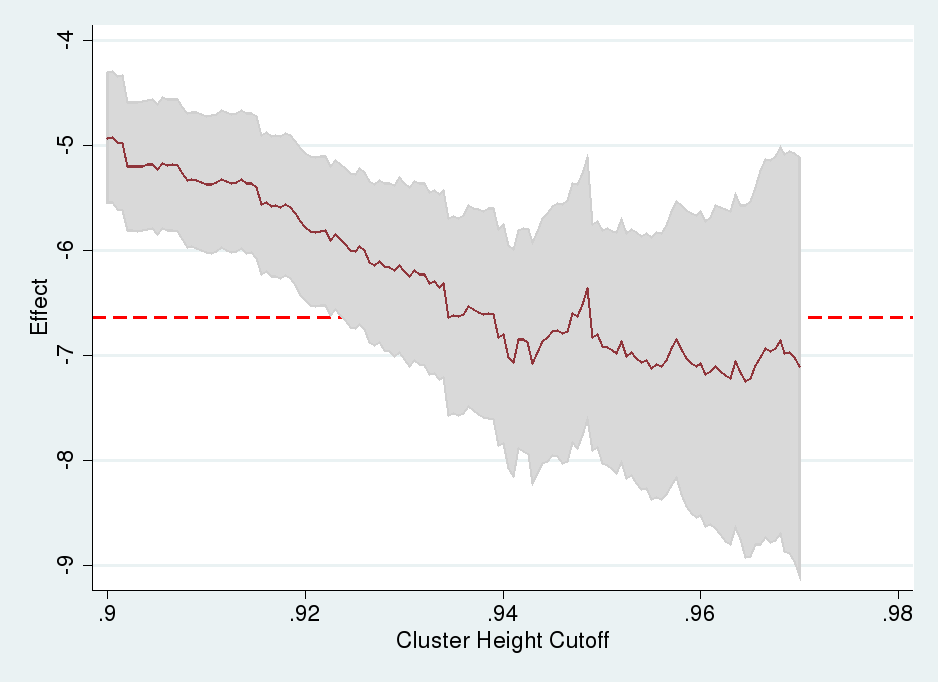
\includegraphics[scale=.35]{./figures/cutoff_bartik.png} \\ 

\multicolumn{1}{p{6.5in}}{\footnotesize \emph{Note:} Author's estimates of $\beta$ in Equation \ref{eqn:bartikreg} based on replication of Tolbert and Sizer's method while varying the cluster height cutoff. The solid red line gives the point estimate for the cluster definitions at each height and the gray area denotes the 90 percent confidence interval including the estimate. The red dashed line gives the point estimate for clusters using the definition FKV1990.}
\end{tabular}
\end{figure}

Figure \ref{fig:cutoff_dist} displays the results of this exercise. Again, our results show that there is some variation in the estimate based on the cutoff value. As the cutoff increases (and there are fewer areas) the effect becomes more negative. However, the relationship is not monotonic.

\subsection{Sensitivity to Errors in Flows Data}

To demonstrate how sensitive the results of Equation \ref{eqn:bartikreg} are to different commuting definitions, we re-estimate the equation using the 1000 realizations of commuting zones that were generated in the previous section.

\begin{figure}\centering
\caption{Distribution of Effect \label{fig:1990dist}}
\begin{tabular}{c}
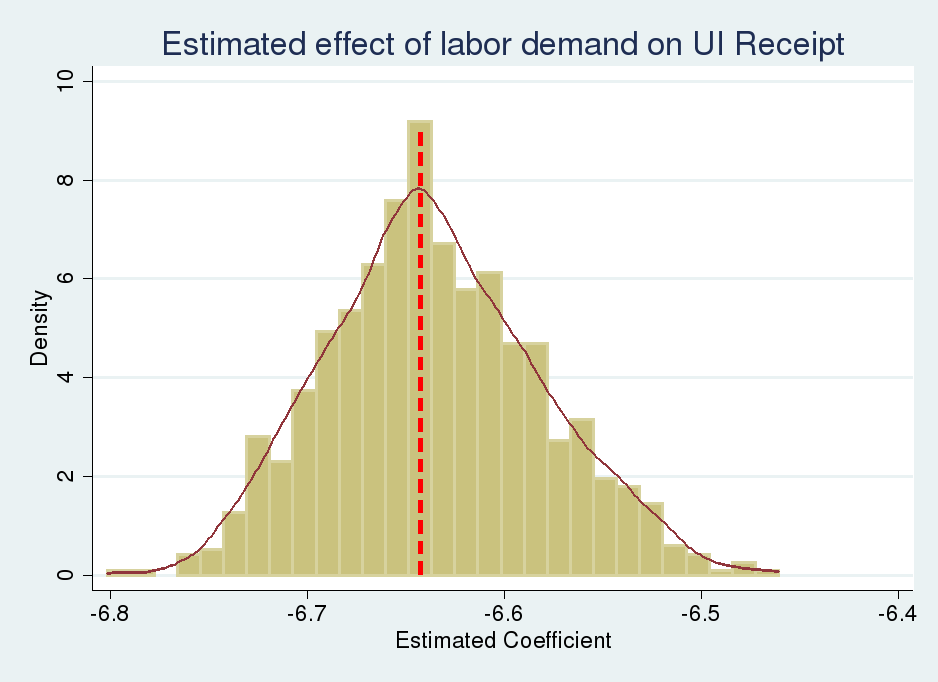
\includegraphics[scale=.35]{./figures/beta_bartik_distribution_moe_new.png}\\
\multicolumn{1}{p{4.5in}}{\footnotesize \emph{Note:} Histogram plots estimates of $\beta_1$ from equation \ref{eqn:bartikreg}, based on commuting zone realizations as outlined in Section \ref{sec:dsens}. Red vertical line shows estimates using replicated commuting zones.}
\end{tabular}
\end{figure}

 The coefficients from this exercise are graphed in Figure \ref{fig:1990dist}, which shows the distribution of the estimated effect from our exercise. The red vertical line shows the estimate using the published flows data from our national replication. Approximately 95 percent of the estimates are within 0.1 of the point estimate -6.643 for FKV1990.

Another way to summarize the results of this exercise is to look at the distribution of t-statistics, which incorporates information about the standard error of $\beta$ into the analysis as well, and comparing that distribution to the critical values. To use the distribution of t-statistics in an empirical setting, researchers construct a 95\% confidence interval of the t-statistic by using the values at the 97.5th and 2.5th percentiles of the 1000 realizations. If this confidence interval is outside the critical value $t_{0.025}$, then the null hypothesis can be rejected at $\alpha = 0.05$. 

To give an empirical application, Figure \ref{fig:1990_tdist} shows the distribution of t-statistics obtained from estimating Equation \ref{eqn:bartikreg}. The blue vertical line is the original t-statistic, and the light gray vertical lines are the 2.5th and 97.5th percentiles. Clearly, in this application the result is still significant, because the entire confidence interval of t-statistics is less than the critical value ($-1.96$). Once again, the t-statistic from the original estimate is one of the smallest in magnitude.

Importantly, the estimated t-statistic from the original regression (blue vertical line) is not the center of the distribution. While this is not true in all applications, it warrants caution on the part of the researcher, because the zones that are used by the researcher may represent an outlier in terms of statistical significance.

\begin{figure}\centering
\caption{Distribution of T-Statistic \label{fig:1990_tdist}}
\begin{tabular}{c}
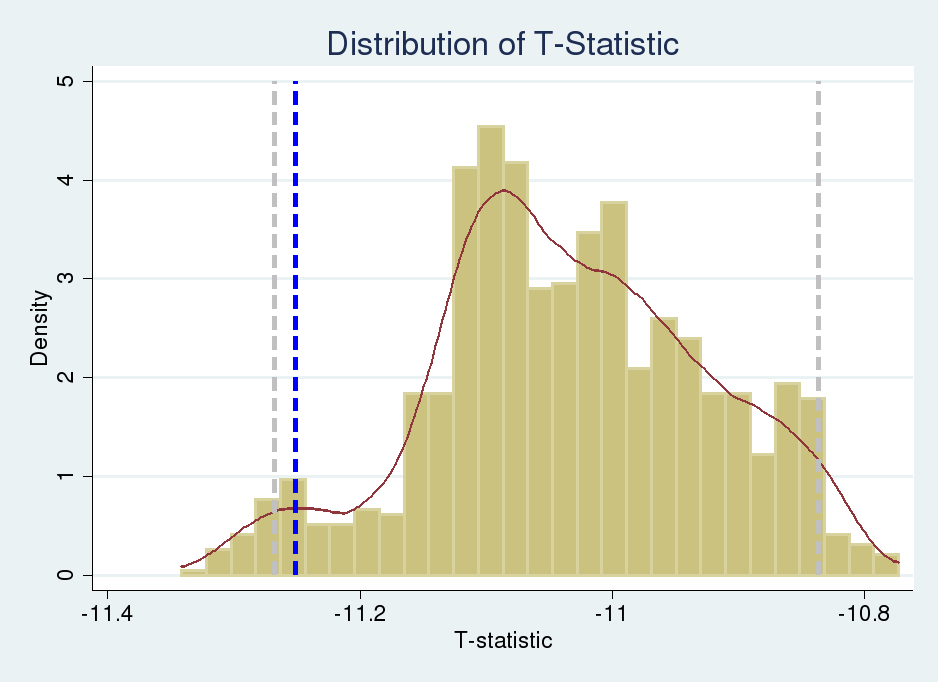
\includegraphics[scale=.35]{./figures/tdistribution_bartik_moe_new.png}\\
\multicolumn{1}{p{4.5in}}{\footnotesize \emph{Note:} Histogram plots t-statistics derived from estimating  equation \ref{eqn:bartikreg}, based on commuting zone realizations as outlined in Section \ref{sec:dsens}. Blue vertical line is t-statistic using FKV1990, and gray vertical lines are the 2.5th and 97.5th percentiles of the t-statistic distribution.}
\end{tabular}
\end{figure}

This exercise demonstrates that there is additional uncertainty induced by the construction of the commuting zones that is not addressed in empirical estimates that use these definitions, which may overstate the precision of the results.







%%%%%%%%%%%%%%%%%%%%%%%%%%%%%%%%%%%%%%%%%%%
\section{Conclusion \label{sec:conclusion}}

From the results above, it is clear that current commuting zone definitions understate the uncertainty of zone assignment, which has implications for empirical results. Importantly, this uncertainty manifests itself on two different margins: uncertainty about zone assignment due to errors in the flows, and uncertainty about zone assignment due to the chosen cutoff. 

Given this uncertainty, we have two pieces of advice for researchers using commuting zones. First, we suggest displaying results for a variety of different cluster counts resulting from a range of cutoff values. This point is particularly important for researchers applying the methodology from TS to new datasets or for characterizing labor markets outside the United States, given that cluster counts are subjective and that results can differ considerably based on the count. Second, we suggest re-estimating results using multiple realizations of commuting zones, which incorporates the additional uncertainty because of the underlying error in the measurement of flows. Researchers can validate results by examining either the distribution of $\beta$ or the distribution of the t-statistics, as described in the previous sub-sections. 

To aid researchers in this effort, we provide datasets and code online that include a crosswalk from county to all the realizations of commuting zones used in this paper to characterize uncertainty in inputs as as well as different cutoff values.\footnote{Our code is available at \iftoggle{blind}{[URL suppressed]}{\url{https://github.com/larsvilhuber/MobZ/}}, see also \iftoggle{blind}{[self-citation suppressed]}{\citet{mobzrepl201704}}.} We also provide our sample code that produced Figures \ref{fig:1990dist} and \ref{fig:cutoff_dist}.

Numerous influential papers in labor economics have used commuting zones as an alternative definition to local labor markets. However, researchers typically do not evaluate how the methodology used to construct commuting zones may impact their findings, nor have there been any evaluations of the sensitivity of commuting zones to design feature more generally. Our paper contributes to this literature by analyzing this methodology and its implications for empirical applications.

We document that the commuting zone methodology is sensitive to uncertainty in the input data and parameter choices and we demonstrate how these features affect the resulting labor market definitions. Furthermore, we demonstrate that uncertainty in local labor market definitions also affects empirical estimates that use commuting zones as a unit of analysis. 

Future work may explore other clustering methods, which are less history-dependent, as they may be better suited for considering a wide range of cluster counts and for evaluating the optimality of cluster counts. Developing metrics to compare zone configurations against one another will facilitate comparisons of the overlap of different clustering outcomes. A more complete characterization of measurement error in the flow measures, reflecting the sparse nature of survey responses, may improve the economic interpretation of flows in rural areas and for long distance flows. Additional metrics of local labor market integration may help to evaluate the overall validity of various definitions.



%%%%%%%%%%%%%%%
% BIBLIOGRAPHY
%%%%%%%%%%%%%%%
\clearpage
\singlespacing

\bibliographystyle{aea}
\bibliography{bibliography}

\newpage
\appendix
\section*{Tables and Figures Appendix}
\FloatBarrier

\appendix
\setcounter{table}{0}
\renewcommand{\thetable}{A\arabic{table}}   
\setcounter{figure}{0}
\renewcommand{\thefigure}{A\arabic{figure}}   

\begin{figure}[th]
\caption{Various Height Cutoffs for California \label{fig:caliclusters}}
\begin{tabular}{cc}
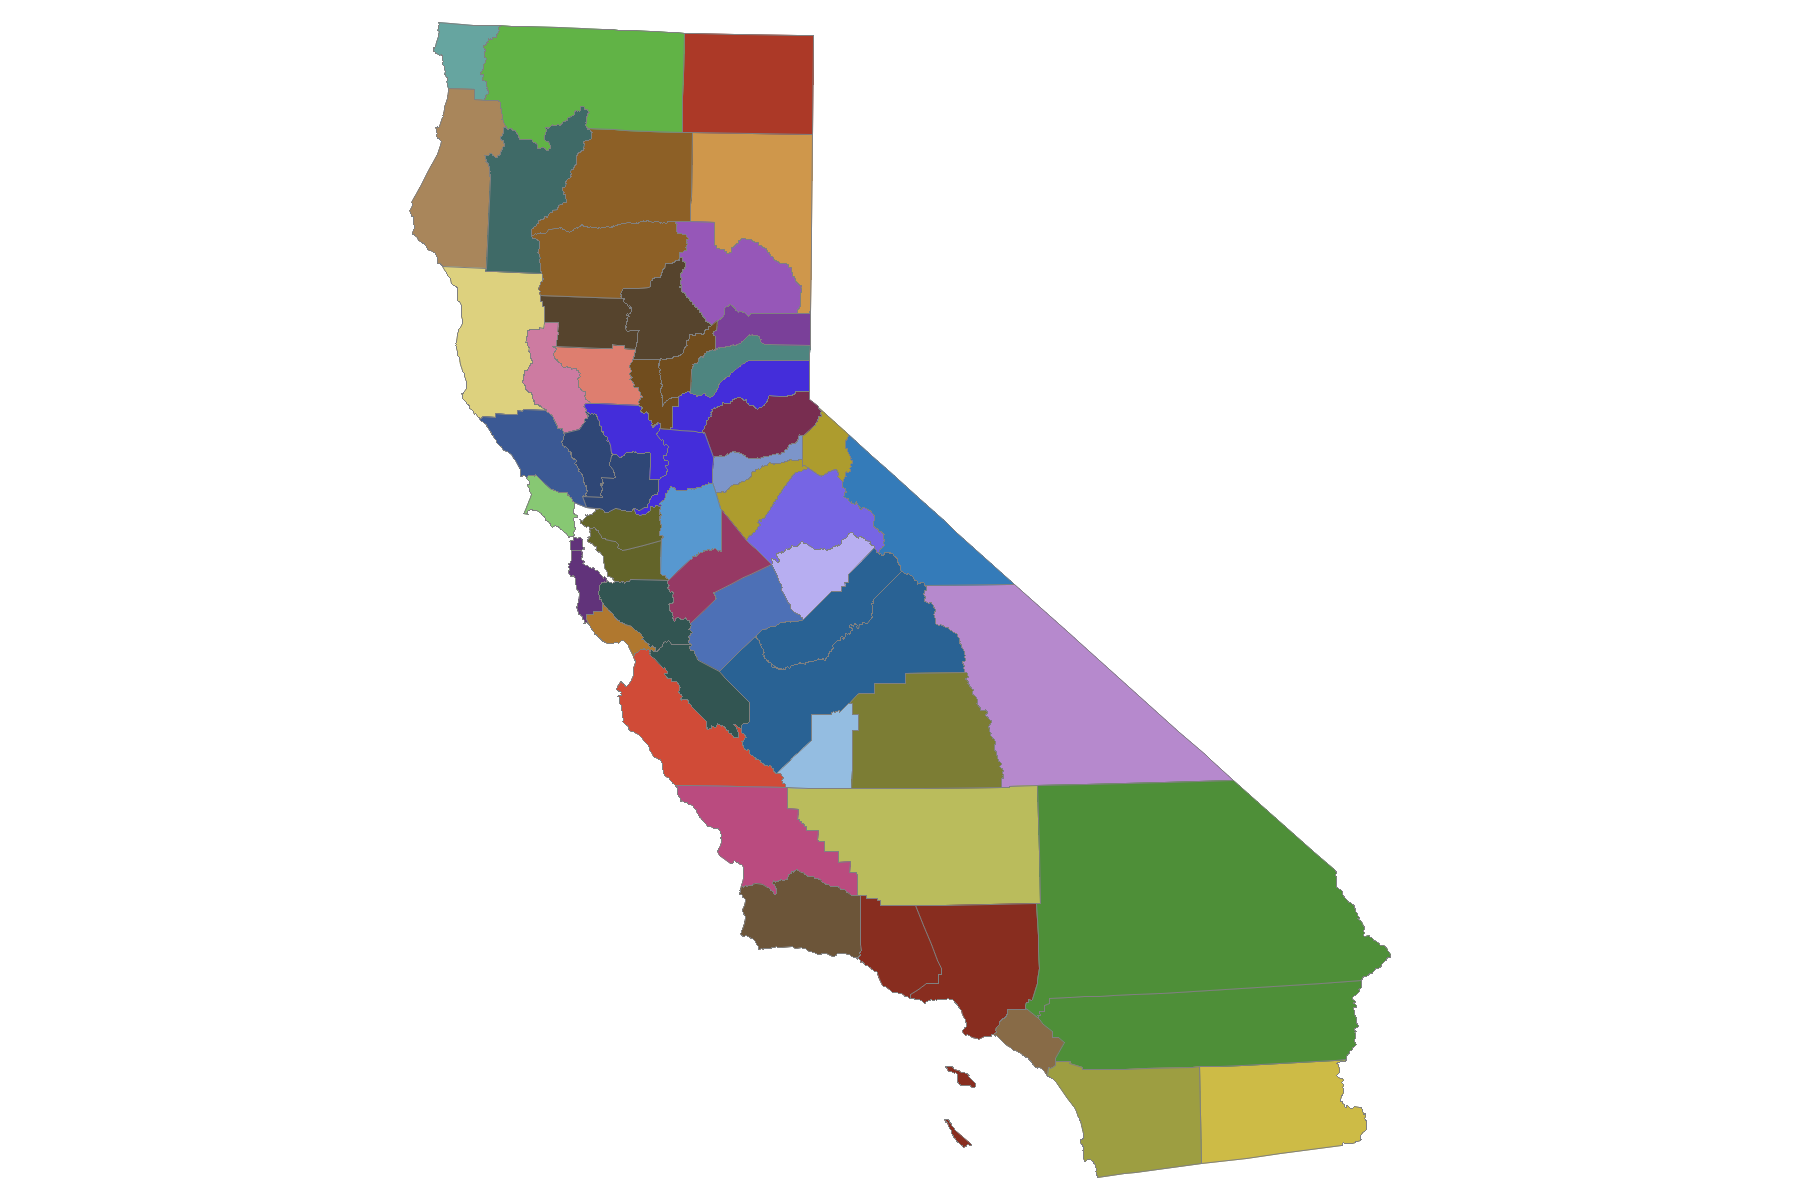
\includegraphics[scale=0.1]{./figures/insetmaps/california_clustermap_800_inset6.png} & 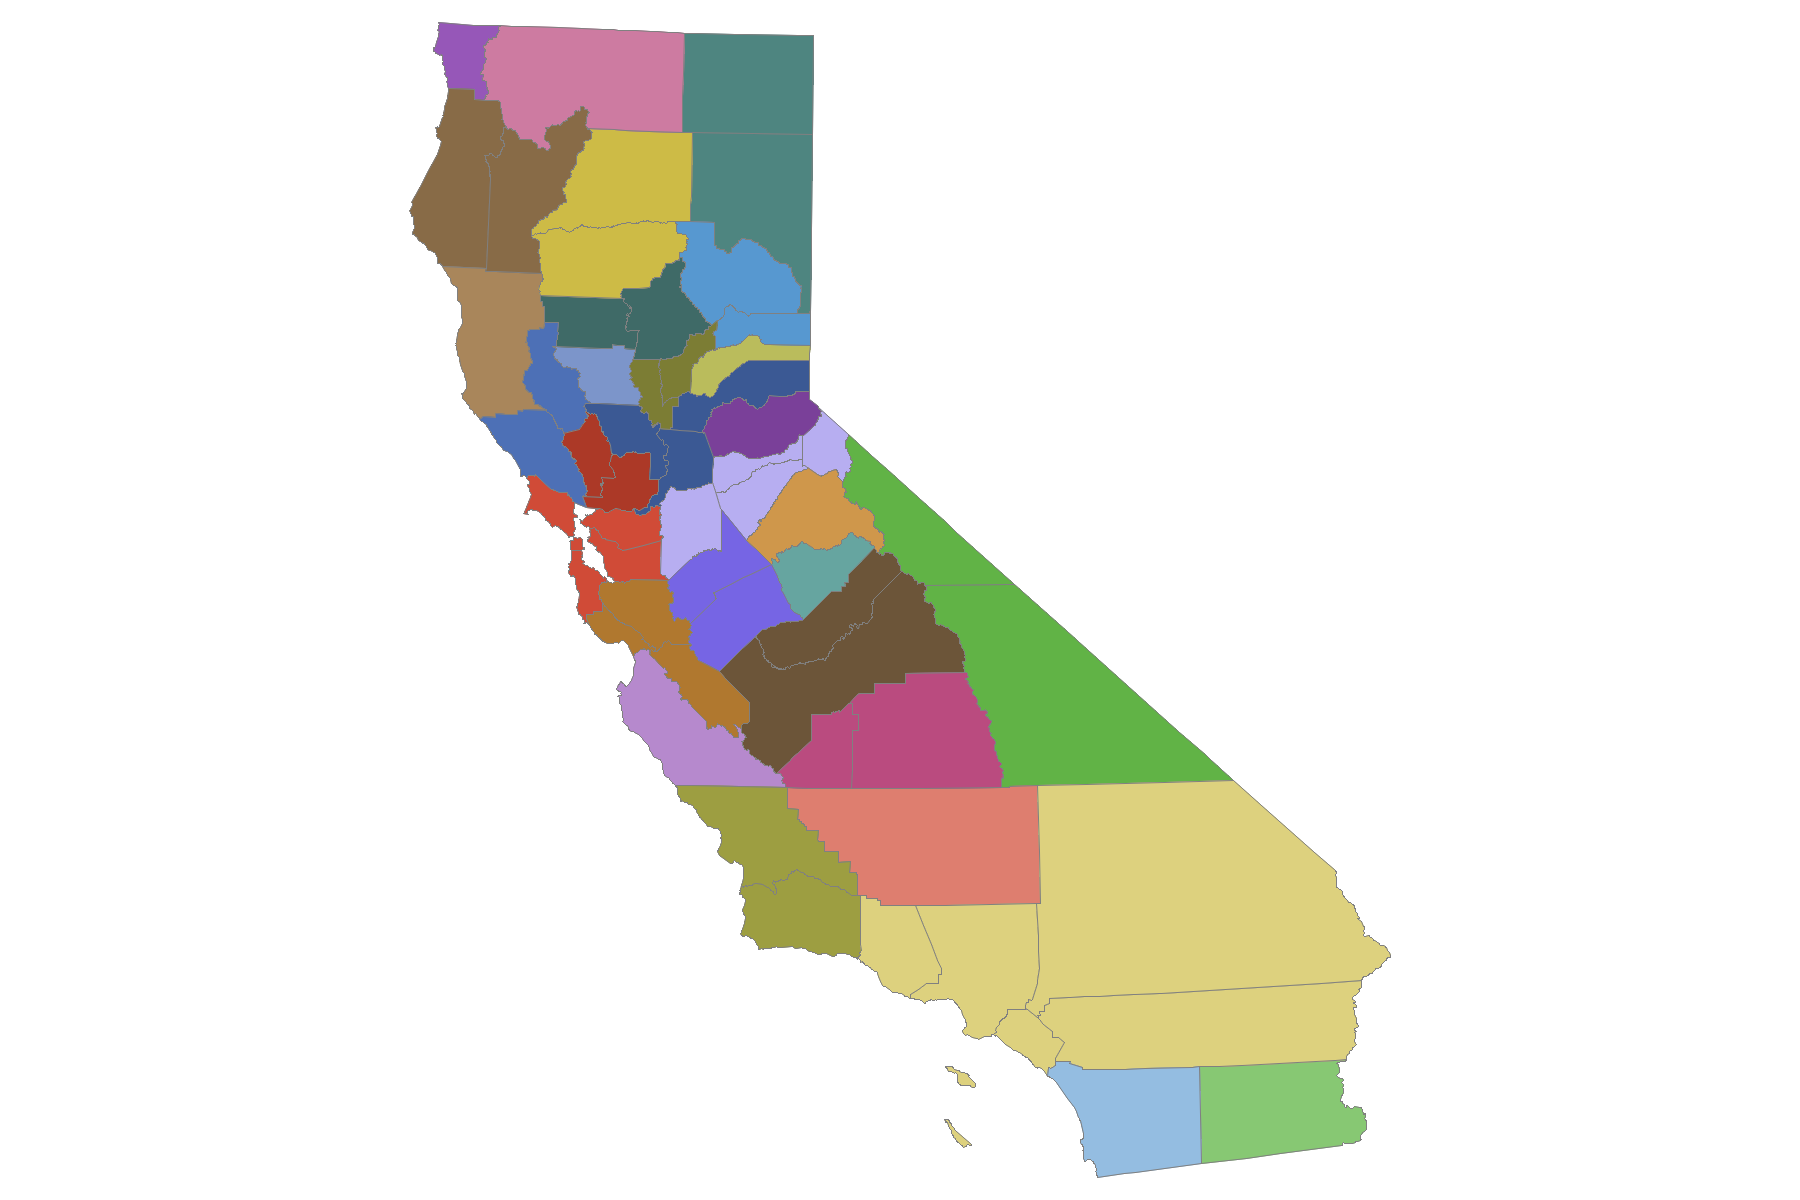
\includegraphics[scale=0.1]{./figures/insetmaps/california_clustermap_880_inset6.png} \\
Height = 0.8 & Height = 0.88 \\
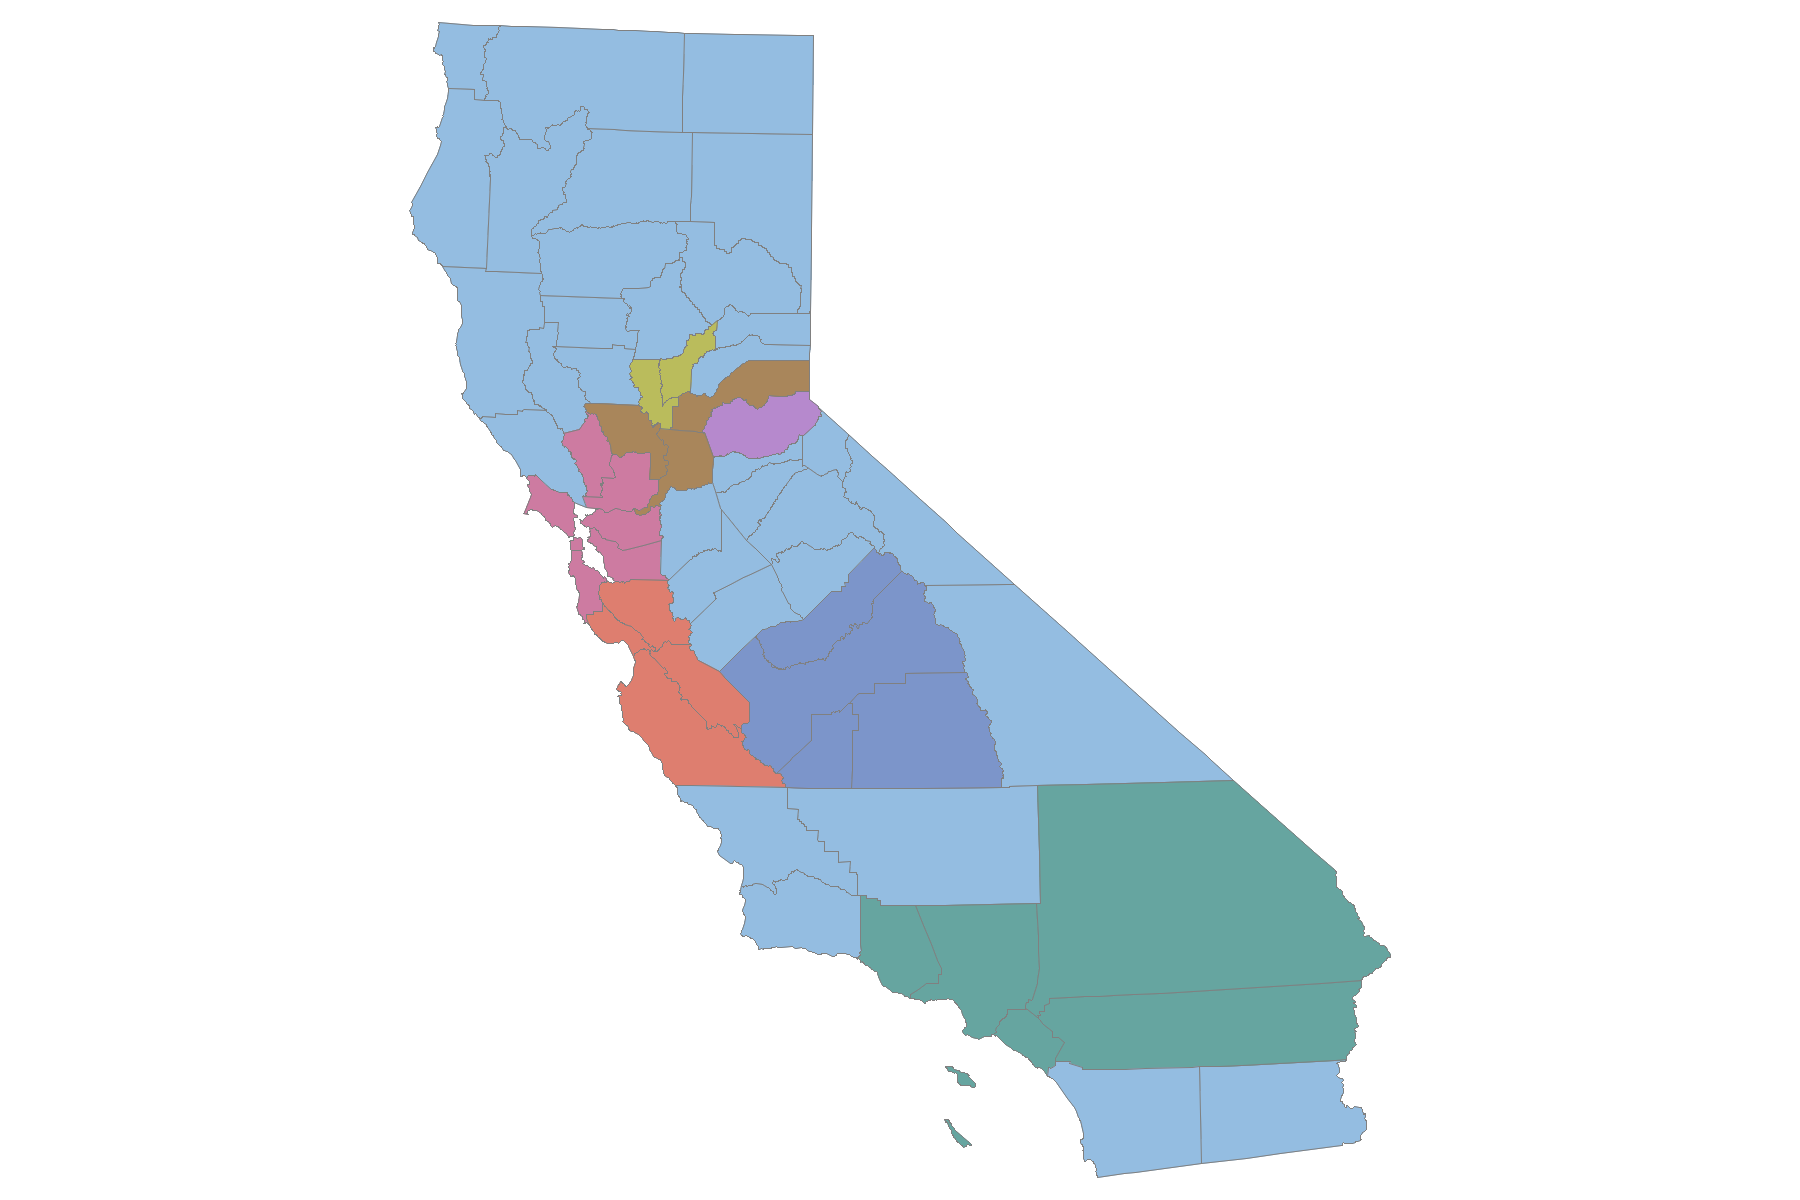
\includegraphics[scale=0.1]{./figures/insetmaps/california_clustermap_960_inset6.png} & 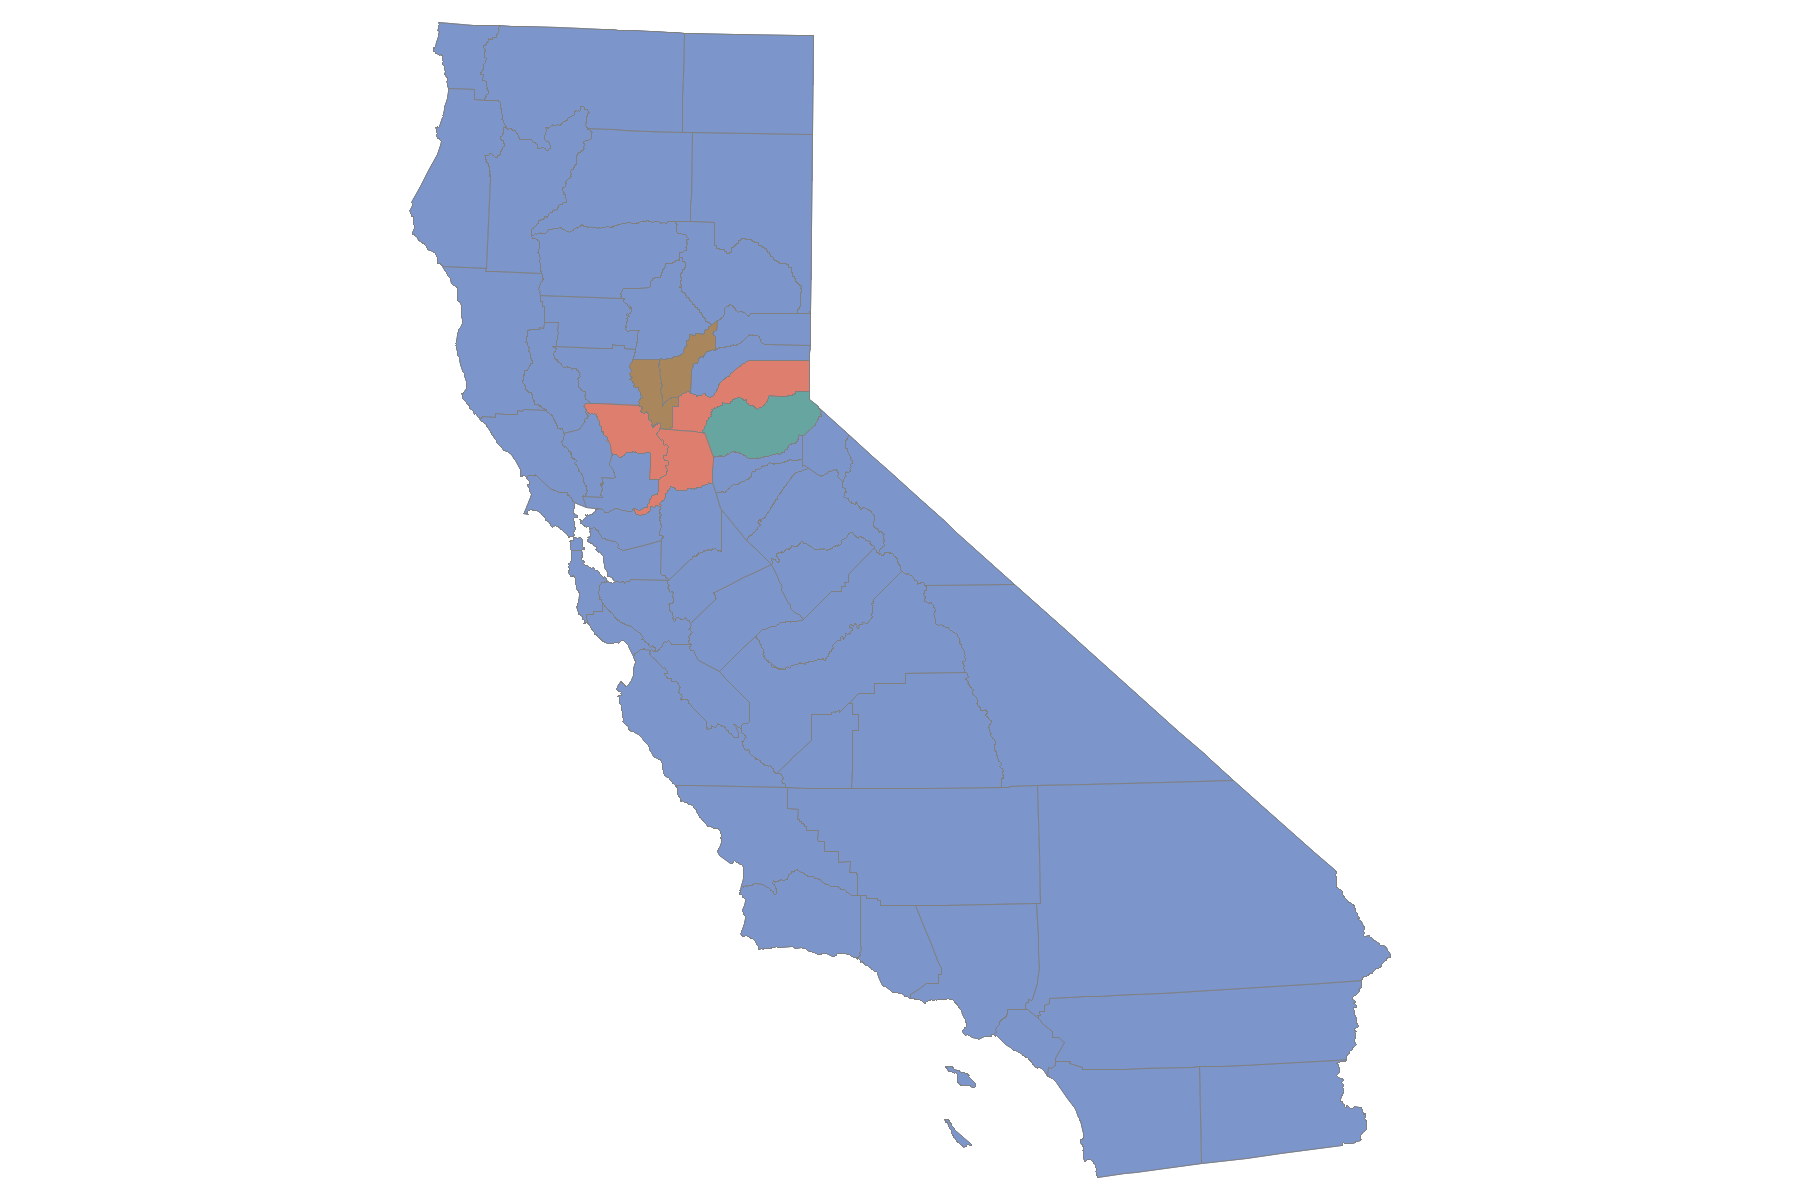
\includegraphics[scale=0.1]{./figures/insetmaps/california_clustermap_1000_inset6.png} \\
Height = 0.96 & Height = 1\\
\multicolumn{2}{p{5in}}{\footnotesize \emph{Notes:} The above graphs are generated using the methodology outlined in Section \ref{sec:method}, using 1990 Census JTW data. More detail is in the text.}
\end{tabular}
\end{figure}


\begin{figure}[th]
\caption{Heirarchical Clustering, Cutoff = 0.945 \label{fig:highcutoff}}
\begin{tabular}{c}
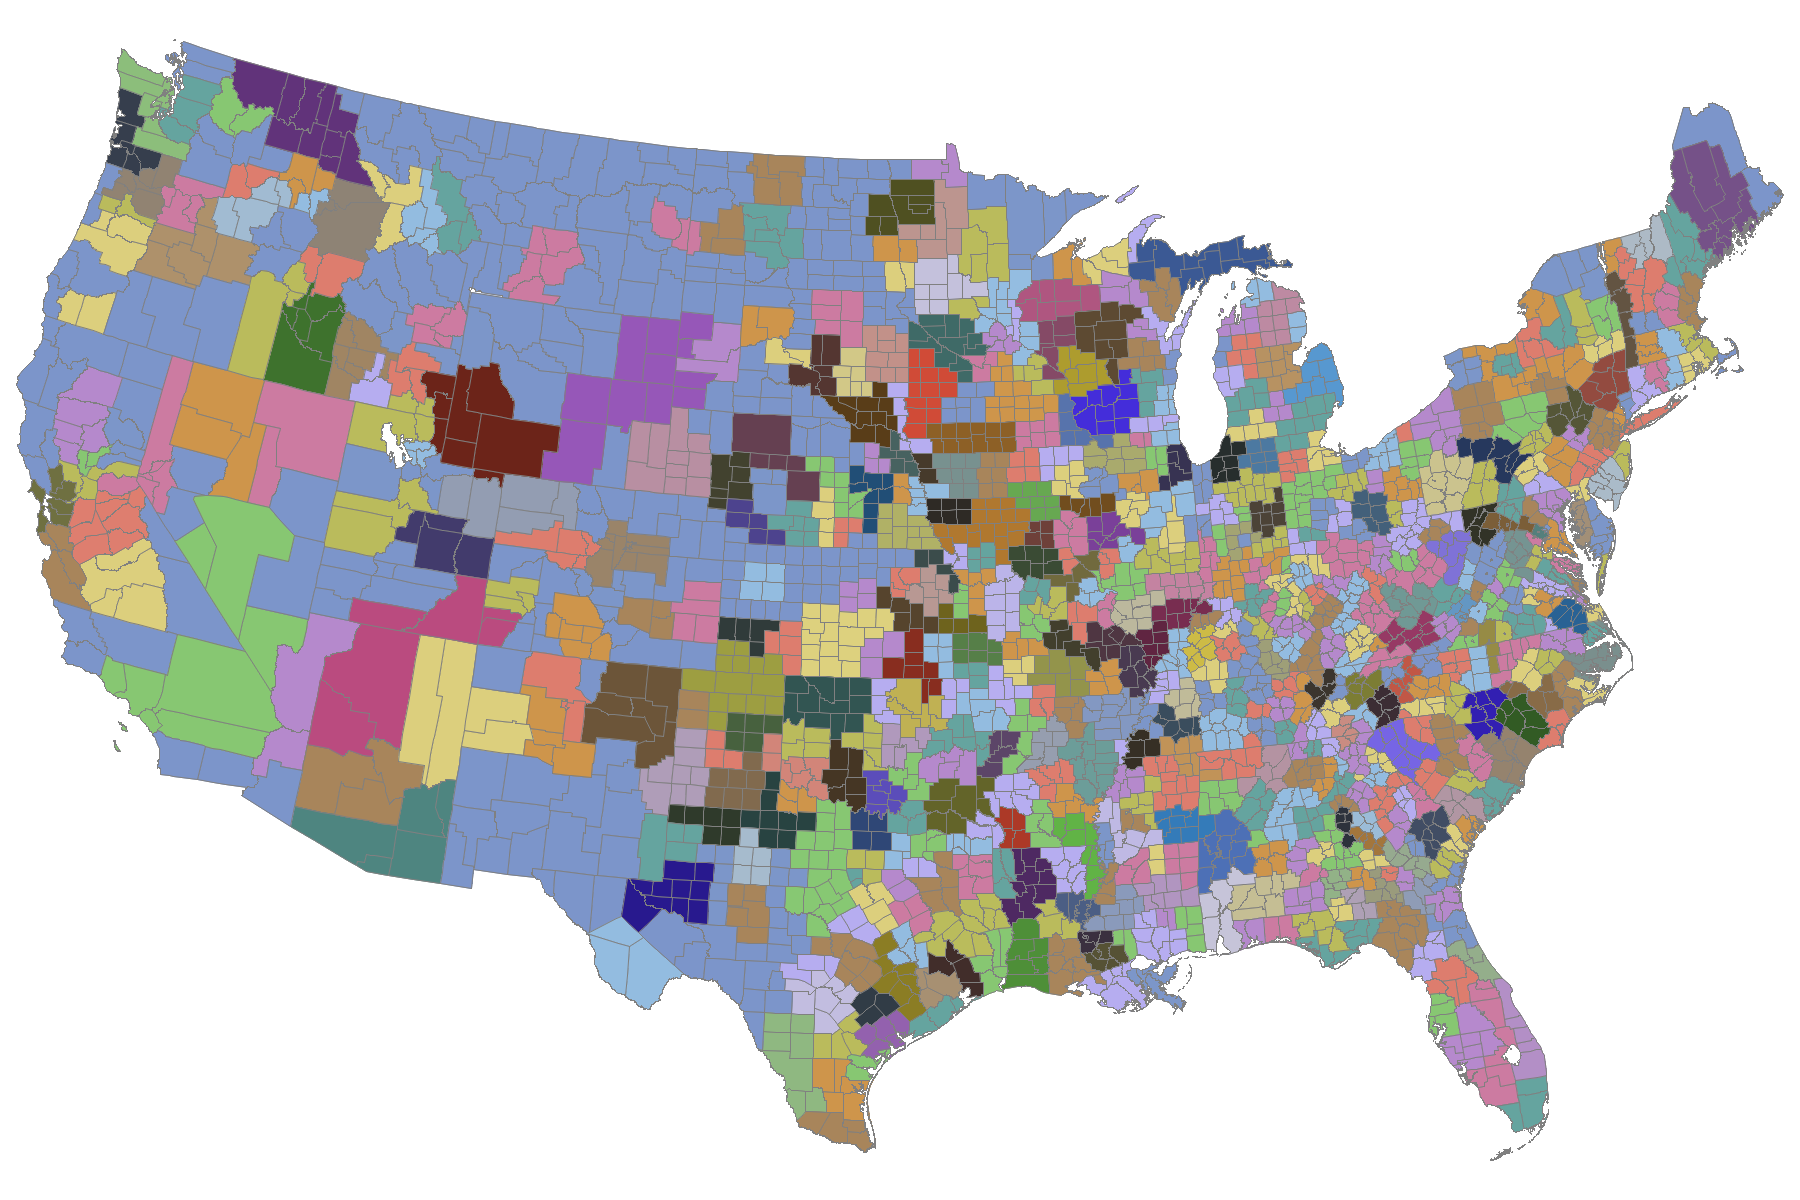
\includegraphics[scale=0.3]{./figures/jtw1990_highcutoff.png}  \\
\multicolumn{1}{p{5in}}{\footnotesize \emph{Notes:} The above graph was generated using the methodology outlined in Section \ref{sec:method}, using 1990 Census JTW data, with a height cutoff of 0.945. All the blue counties are in the same cluster, even though parts of the cluster are non-contiguous; there are 292 counties in that cluster.}
\end{tabular}
\end{figure}

\begin{table}[h]
\caption{Summary Statistics of Ratio of MOE to Flows \label{tab:moesum}}
\begin{tabular}{lcccc}
\hline\hline
& Mean & 25th Pctile & 50th Pctile & 75th Pctile \\
\hline
All counties & 1.236 & 0.845 & 1.370 & 1.600\\
Flows <100 & 1.432 & 1.148 & 1.500 & 1.636 \\
Flows 100-1000 & 0.444 & 0.301 & 0.414 & 0.549  \\
Flows 1000-10000 & 0.131 & 0.087 & 0.124 & 0.169 \\
Flows 10000+ & 0.037 & 0.024 & 0.036 & 0.049 \\
\hline\hline
\multicolumn{5}{p{4in}}{\footnotesize \emph{Notes:} Author's calculation using
2009-2013 ACS Journey-to-Work data.}
\end{tabular}
\end{table}

\begin{table}
\caption{Summary statistics for empirical example}
\begin{tabular}{lcc}
\hline\hline 
	& TS 1990 CZs & Replicated CZs \\
Log UI receipts & 9.23     &  9.59   	\\
				& (1.89)	&  (1.54)	\\
$Bartik_{it}$	& 0.006		&	0.006		\\
				& (0.022)		&	(0.022)		\\
                \hline	
\multicolumn{3}{p{4in}}{\footnotesize \textit{Notes:} For details on construction and source, see Section \ref{sec:esens}. Standard deviations in parentheses.} \\
\hline\hline
\end{tabular}                
\end{table}





\end{document}
